\section{Diffusion Processes}


\subsection{Historical Note}

\par Quantitative analysis of transport phenomena was not entirely described up until 1828 with Thomas Graham's experiments on diffusion in gases and liquids \cite{cussler}. Later that century in 1855, Adolf Fick codified the experiments of Graham in what we now know as Fick's Laws. The First Law of Fick's states that the one dimensional flux of a species $i$(that is, the particles per unit time that move through a certain area) is deifined as \cite{cussler}

\begin{align}
\label{eq:fick-fluxes}
	J_i = A j_i = -A\mathcal{D}_i\frac{\partial c_i}{\partial x},
\end{align}

where $\mathcal{D}_i$ is the diffusion coefficient of the species, $c_i$ is the concentration, $x$ the position, $A$ the cross sectional area. This is known as Fick's first law. Fick was inspired to draw this conclusion from Fourier's work in heat and by the findings of Graham \cite{fick}.


\subsection{Derivation Of Fick's Second Law}

In order to derive Fick's Law for fluxes, we consired diffusion through a thin layer. We want to account for the accumulation of solute within the membrane of Fig. \ref{fig:cussler_thin_layer}. The accumulation should be equal to the rate of diffusion coming into the membrane at $z$ minus the rate at which solute is leaving the membrane at $z+\Delta z$. The sign of the flow is accounted by the fact that particles diffuse from higher concentrations to lower concentrations (from left to right in this case). Therefore,

\begin{align}
	\qty{\textnormal{Solute accumulation in volume }A\Delta z} =& \qty{\textnormal{Diffusive flux at } z } \nonumber\\
	&- \qty{\textnormal{Diffusive flux at } z+\Delta z}.\nonumber
\end{align}


Accumulation is by definition the rate of change of the total mass contained in the sample volume $V = A\Delta z$. Therefore

\begin{align}
	\label{eq:derivation-fick-1}
	\frac{\partial \qty{c_1 A\Delta z}}{\partial t} = \qty{J_1 - J_2}.
\end{align}

Where $J_1$ and $J_2$ are the Fick fluxes at $z$ and $z+\Delta z$. Replacing \ref{eq:fick-fluxes} into \ref{eq:derivation-fick-1} and assuming the cross sectional area $A$ is constant

\begin{align}
	\frac{\partial c_1}{\partial t} = \frac{\qty{j_1 - j_2}}{\Delta z},\\
	\frac{\partial c_1}{\partial t} = -\mathcal{D}\frac{\qty{\frac{\Delta c_1}{\Delta z} - \frac{\Delta c_2}{\Delta z}}}{\Delta z}.
\end{align}

As we take $\Delta z \rightarrow 0$ the last equation reduces to

\begin{align}
\label{eq:second-ficks-law}
	\frac{\partial c}{\partial t} = \mathcal{D}\frac{\partial^2 c}{\partial z^2},
\end{align}

since $c_1\approx c_2 = c$.
\begin{figure}[h!]
\centering
	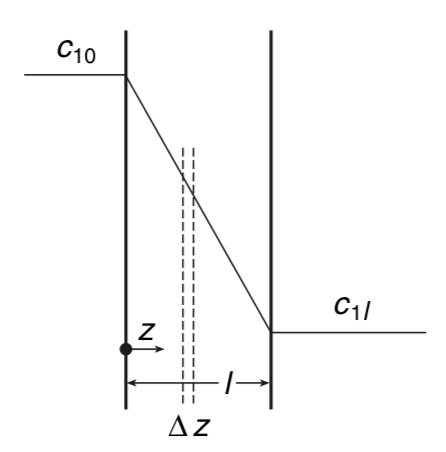
\includegraphics[width=0.5\textwidth]{diffusion_thin_membrane}
	\caption{Diffusion through a thin layer (plot extracted from reference \cite{cussler})}
\label{fig:cussler_thin_layer}
\end{figure}




A particularly interesting solution to equation \ref{eq:second-ficks-law} is that of an initial condition where we have a peak concentration at $x=0$ (such as a drop of substance falling into the underlying fluid at $x=0$). Such initial condition can be stated as

\begin{align}
	c(z,t=0) = n_0 \delta(z),
\end{align}

where $n_0$ is the concentration of substance in the drop and $z$ is the horizontal distance \ref{fig:cussler_thin_layer}. The solution to Ficks law is then

\begin{align}
	\label{eq:solution-fick}
	n(z,t) = \frac{2n_0}{\sqrt{\pi}}\int_0^z e^{-\frac{x^2}{4\mathcal{D}t}}dx.
\end{align}






\subsection{Diffusion Coefficients}

In 1905 Albert Einstein showed that the diffusion of molecules is due to collisions between the suspended particles and the random molecular motion of the medium in which they are suspended \cite{einstein}. 

To understand the physical nature of the diffusion coefficient, one can imagine the setup in which brownian motion was first observed. Let a pollen particle float on water. By close observation with a microscope one finds that the particle starts to move erratically around the center. Nowadays this problem can be studied under the theoretical framework of diffusion of polymers \cite{bird}.

Using arguments from thermodynamics and kinetic theory of gases, Einstein calculated the conditions under which the suspended pollen particle would reach equilibrium states, by minimizing Helmholtz free energy. He found that, if a complementary stochastic force $K$ acts upon a system of $\nu$ particles per unit volume, then at equilibrium

\begin{align}
	-K\nu +\frac{RT}{N}\frac{\partial \nu}{\partial z} = 0.
\end{align} 

Recognizing that osmotic pressure is $p = RT \nu /N$ we get

\begin{align}
\label{eq:einstein-result}
	K\nu - \frac{\partial p}{\partial z} = ,
\end{align}

which shows that equilibrium with force $K$ is brought by osmotic pressure \cite{einstein}. 

With these considerations, we can conclude that the amount of flux produced by the stochastic force $K$ applied to perfectly spherical particles of radius $r$ is

\begin{align}
	\label{flux}
	j(x) = -\frac{\nu K}{6\pi u r},
\end{align}

where u is the viscosity of the fluid. From Fick's law the total flux is given by

\begin{align}
	\label{flux-def}
	j(x) = -\mathcal{D}\frac{\partial \nu}{\partial z}.
\end{align}

Replacing $\nu$ from Eq. \ref{eq:einstein-result} and equation Eqs. \ref{flux-def} and \ref{flux}.

\begin{align}
\frac{\nu K}{6\pi u R} = \mathcal{D}\frac{N}{RT}\nu K,
\end{align}

Finally, for spherical colloids of radius $R$

\begin{align}
	\mathcal{D} = \frac{RT}{6N\pi u r}.
\end{align}


This is known as the Stokes-Einstein equation and it gives us a physical understanding of how the coefficients fluctuate with temperature and particle size. It is known that this is acurrate to only 20\%, but is still the standard to compute diffusivity coefficients (\cite{cussler}, page 127).









\subsection{Langevin Equation}

Langevin proposed the motion equations for the polymers in suspention \cite{langevin_translation}. He proposed that, based on the equipartition of kinetic energy among the degrees of freedom of a particular system, the average speed of the particles in the system in a one dimensional setting, from the equipartition of energy

\begin{align}
	\frac{1}{2}m\bar{v}^2 = \frac{RT}{2N}.
\end{align}

If the suspended particles are big enough (that is, much larger than the average distance between molecules in the fluid) then the particle is subjected to a viscous resistance proportional to the speed of the particle itself

\begin{align}
	\label{eq:friction}
	F_r(x) = -6\pi\nu r \bar{v},
\end{align}

where $\nu$ is the viscosity and $r$ the radius of the colloid. This however, is an approximation \cite{langevin_original}. Due to impacts of the fluid's constitutive particles the action of the particle oscillates about the value \ref{eq:friction}. Thus, the motion equation of the particle suspended in liquid is

\begin{align}
\label{eq:langevin}
	m\frac{d v}{dt} = -6\pi\nu r v(t) + K(t),
\end{align}

where K is a complementary force induced by the random movement of the particles composing the fluid. This is known as the Langevin equation. 


To gain physical insight of this equation, Langevin \cite{langevin_original} set out to find the variance of the displacement ($\Delta_x^2$) of the particle suspended in liquid. 

The following method is what he used to find $\Delta_x^2$. Multiplying by x and writing
\begin{align}
	\frac{d}{dt}x^2 = 2x\frac{dx}{dt},\\	
	\frac{d^2}{dt^2}x^2 = 2\qty{x\frac{d^2x}{dt^2}+\qty{\frac{dx}{dt}}^2}
\end{align}


we get the equation

\begin{align}
	\frac{m}{2}\qty{\frac{d^2x^2}{dt^2} - 2\qty{\frac{dx}{dt}}^2} = -3\pi\nu r \frac{d x^2}{dt} + K(t)x.
\end{align}

Averaging out the later equation (with the bar symbol as the average notation), we obtain the term $<Kx>$. To get rid of this term, we consider that the complementary force $K$ should come from no prefered direction (kicks from the liquid particles come from every direction), we get $<Kx> = 0$. Considering also the fact that

\begin{align}
	m\left<\qty{\frac{d x}{dt}}^2\right> = \frac{RT}{N}.
\end{align}

Equation \ref{eq:langevin} yields

\begin{align}
	\frac{m}{2}\frac{d^2\bar{x^2}}{dt^2} + 3\pi\nu r \frac{d \bar{x^2}}{dt} = \frac{RT}{N}.
\end{align}

Replacing $z = d\bar{x^2}/dt$ we get

\begin{align}
	\frac{m}{2}\frac{dz}{dt}(z) + 3\pi\nu r z(t) = \frac{RT}{N}.
\end{align}

This equation can be solved for $z$

\begin{align}
	\label{eq:sol-to-langevin}
	z(t) = \frac{RT}{N}\frac{1}{3\pi\nu r} + Ce^{-\frac{6\pi\nu r}{m}t}.
\end{align}

Note from \ref{eq:sol-to-langevin} that the system reaches a steady regime for large $t$. In this regime, we can solve

\begin{align}
	z = \frac{d \bar{x^2}}{dt} =  \frac{RT}{N}\frac{1}{3\pi\nu r},
\end{align}

which gives us

\begin{align}
	\bar{\Delta_x^2} = \bar{x^2} - \bar{x_0^2} =  \frac{RT}{N}\frac{\Delta t}{3\pi\nu r},
\end{align}

where $\Delta t$ is the interval which we are measuring ($t-t_0$), with $t_0$ is the initial time. This is the famous result from Langevin \cite{langevin_original}.











\subsection{Diffusion of Electrolytes}

In electrolyte diffusion, other forces must be taken into account in order to provide an accurate model. This is because of two reasons: One, diffusion of electrolytes is diffusion of at least two types of particles which ionize when disolved in water. Secondly, these charged particles react to possible external electric fields and the electric field produced by the electrolytes themselves.

We know that the flux is given by Fick's law, but this law does not account for the interactions with an electric field. A typical model for the flux of charged particles is

\begin{align}
	j= -\mathcal{D}\qty{\nabla c + \frac{c \mathcal{F}}{RT}\nabla \phi},
\end{align}

which, using Fick's law yield


\begin{align}
\label{eq:nernst-planck}
	\frac{\partial c}{\partial t}= \nabla \cdot D\qty{\nabla c + \frac{c \mathcal{F}}{RT}\nabla \phi},
\end{align}


This is called the Nernst-Planck Equation.

Although Eq. \ref{eq:nernst-planck} accounts for how the diffusion process involves electrical forces in the presence of electrolytes, we haven not accounted as to how the electric field changes due to the presence of electrolytes. 
We start from the Poisson Equation which tells us that

\begin{align}
	\nabla^2 \phi = -\frac{\rho}{\epsilon},
\end{align}

where $\rho$ is the charge distribution, $\epsilon = \epsilon_r \epsilon_0$ is the permittivity of the medium, $\epsilon_r$ the relative permittivity with respect of the void's permittivity $\epsilon_0$. In the case of water as the underlying substance, $\epsilon_r = 80.2$ at $T=20^oC$. By definition, the charge distribution should be the amount of the charge per unit volume, therefore

\begin{align}
	\rho(x,t) = \mathcal{F}\sum_{s=\pm} z_sc_s,
\end{align}

where $c_s$ is the concentration of each species, $z_s$ is the valence of each species and $\mathcal{F} = N_ae$ is the Faraday constant which is a measure of the charge per mol of substance and $e$ is the electron charge and $N_a$ is Avogadro's number. $\epsilon$ is the permittivity of water. Therefore, the Poisson equation takes the form

\begin{align}
	\label{eq:poisson-electrolyte}
	\nabla^2 \phi = -\frac{\mathcal{F}}{\epsilon}\sum_{s=\pm} z_sc_s.
\end{align}














